\documentclass{article}\usepackage[]{graphicx}\usepackage[]{xcolor}
% maxwidth is the original width if it is less than linewidth
% otherwise use linewidth (to make sure the graphics do not exceed the margin)
\makeatletter
\def\maxwidth{ %
  \ifdim\Gin@nat@width>\linewidth
    \linewidth
  \else
    \Gin@nat@width
  \fi
}
\makeatother

\definecolor{fgcolor}{rgb}{0.345, 0.345, 0.345}
\newcommand{\hlnum}[1]{\textcolor[rgb]{0.686,0.059,0.569}{#1}}%
\newcommand{\hlsng}[1]{\textcolor[rgb]{0.192,0.494,0.8}{#1}}%
\newcommand{\hlcom}[1]{\textcolor[rgb]{0.678,0.584,0.686}{\textit{#1}}}%
\newcommand{\hlopt}[1]{\textcolor[rgb]{0,0,0}{#1}}%
\newcommand{\hldef}[1]{\textcolor[rgb]{0.345,0.345,0.345}{#1}}%
\newcommand{\hlkwa}[1]{\textcolor[rgb]{0.161,0.373,0.58}{\textbf{#1}}}%
\newcommand{\hlkwb}[1]{\textcolor[rgb]{0.69,0.353,0.396}{#1}}%
\newcommand{\hlkwc}[1]{\textcolor[rgb]{0.333,0.667,0.333}{#1}}%
\newcommand{\hlkwd}[1]{\textcolor[rgb]{0.737,0.353,0.396}{\textbf{#1}}}%
\let\hlipl\hlkwb

\usepackage{framed}
\makeatletter
\newenvironment{kframe}{%
 \def\at@end@of@kframe{}%
 \ifinner\ifhmode%
  \def\at@end@of@kframe{\end{minipage}}%
  \begin{minipage}{\columnwidth}%
 \fi\fi%
 \def\FrameCommand##1{\hskip\@totalleftmargin \hskip-\fboxsep
 \colorbox{shadecolor}{##1}\hskip-\fboxsep
     % There is no \\@totalrightmargin, so:
     \hskip-\linewidth \hskip-\@totalleftmargin \hskip\columnwidth}%
 \MakeFramed {\advance\hsize-\width
   \@totalleftmargin\z@ \linewidth\hsize
   \@setminipage}}%
 {\par\unskip\endMakeFramed%
 \at@end@of@kframe}
\makeatother

\definecolor{shadecolor}{rgb}{.97, .97, .97}
\definecolor{messagecolor}{rgb}{0, 0, 0}
\definecolor{warningcolor}{rgb}{1, 0, 1}
\definecolor{errorcolor}{rgb}{1, 0, 0}
\newenvironment{knitrout}{}{} % an empty environment to be redefined in TeX

\usepackage{alltt}
\usepackage{amsmath} %This allows me to use the align functionality.
                     %If you find yourself trying to replicate
                     %something you found online, ensure you're
                     %loading the necessary packages!
\usepackage{amsfonts}%Math font
\usepackage{graphicx}%For including graphics
\usepackage{hyperref}%For Hyperlinks
\usepackage[shortlabels]{enumitem}% For enumerated lists with labels specified
                                  % We had to run tlmgr_install("enumitem") in R
\hypersetup{colorlinks = true,citecolor=black} %set citations to have black (not green) color
\usepackage{natbib}        %For the bibliography
\setlength{\bibsep}{0pt plus 0.3ex}
\bibliographystyle{apalike}%For the bibliography
\usepackage[margin=0.50in]{geometry}
\usepackage{float}
\usepackage{multicol}

%fix for figures
\usepackage{caption}
\newenvironment{Figure}
  {\par\medskip\noindent\minipage{\linewidth}}
  {\endminipage\par\medskip}
\IfFileExists{upquote.sty}{\usepackage{upquote}}{}
\begin{document}

\vspace{-1in}
\title{Lab 7/8 -- MATH 240 -- Computational Statistics}

\author{
  Danny Molyneux \\
  Colgate University  \\
  Mathematics  \\
  {\tt dmolyneux@colgate.edu}
}


\maketitle

\begin{multicols}{2} \raggedcolumns
\begin{abstract}
In labs 7 and 8, I did a thorough analysis of the beta distribution. This includes an analysis of its parameters, properties, what it looks like, and what it's used for. This information is helpful for the same reason it would be helpful for any probability distribution. They are a way for us to estimate various properties of data that approximately follows a certain probability distribution.
\end{abstract}

\noindent \textbf{Keywords:} Probability, moments, summarize, sample size.

\section{Introduction}
In this lab, there is not one specific question we want to answer. We more so want to analyze the beta distribution by looking at its use, meaning, parameters, properties, and what it looks like.

We analyze the distribution and its parameters by using multiple sets of parameters, and comparing their plots as well as their numerical summaries. To analyze the properties of the beta distribution, we first see how the mean, variance, skew, and kurtosis vary based on the sample size, and whether or not they converge to the true population values. If you want to see the distribution of these statistics, called sampling distributions, we can do what's called resampling, and store each statistic for every sample we take. 

Another question we aim to answer at the end of the lab is which estimators we should use for the beta distribution, method of moments, or maximum likelihood estimates? We can do this through the use of sampling distributions again, but now for the MOM and MLE for each new sample. I used data on country death rates from 2022 as an example. Calculating properties like bias, precision, and mean squared error can tell us which estimator is more optimal. 

\section{Density Functions and Parameters}
The beta distribution is a continuous distribution that is used to model a random variable that ranges from 0 to 1, meaning it good at modeling probabilities/proportions. It has two parameters, alpha and beta, which are both positive numbers. These parameters affect the distribution's shape, making it very flexible. Let's look more closely at what each of these parameters really means, and what this distribution looks like generally.
pdf 
  2 

\begin{figure} [H]
\centering
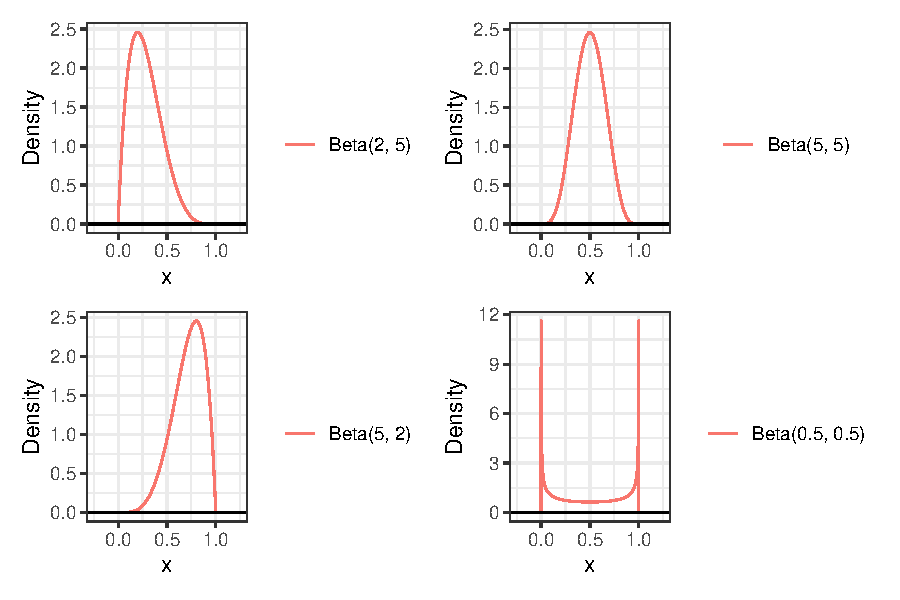
\includegraphics[width=\linewidth]{beta.plots.pdf}
\caption{Histograms for various beta distributions}
\label{fig:beta}
\end{figure}

\begin{table}[H]
\centering
\resizebox{0.4\textwidth}{!}{ 
  \begin{tabular}{rllllll}
    \hline
  & alpha & beta & mean & variance & skew & kurt \\ 
    \hline
  1 & 2.0 & 5.0 & 0.2857143 & 0.02551020 & 0.5962848 & -0.1200000 \\ 
  2 & 5.0 & 5.0 & 0.5000000 & 0.02272727 & 0.0000000 & -0.4615385 \\ 
  3 & 5.0 & 2.0 & 0.7142857 & 0.02551020 & -0.5962848 & -0.1200000 \\ 
  4 & 0.5 & 0.5 & 0.5000000 & 0.12500000 & 0.0000000 & -1.5000000 \\
    \hline
  \end{tabular}
}
\caption{Numerical summaries of beta distributions} 
\label{beta.plots:reference}
\end{table}

As you can see, I made plots for each of the four distributions using the ggplot2 *** and tidyverse *** packages. The Beta(2,5) plot is skewed left, and the Beta(5,2) plot is the same graph, except skewed right. When alpha and beta are equal (5,5), the plot is symmetrical. This tells me that having a larger alpha skews the graph right, and a larger beta skews the graph left. What this means is that a larger alpha means more data will be near 1, indicating that alpha represents "successes". We can say the opposite about beta. However, you can see in the Beta(0.5,0.5) plot that it has a U-shape. This is because when the parameters are less than 1, the plot becomes bimodal with peaks near 0 and 1. This is just a result due to the probability density function of the Beta distribution. One thing to note from the table if you couldn't tell from the plots is that the mean is 0.5 if alpha and beta are equal. If alpha is larger, the mean is closer to one, and the opposite is true if beta is larger. This makes sense given the skewness we know that the parameters cause.

So now we know that if the two parameters are greater than or equal to one, the Beta distribution will have a bell-shaped curve, with its skewness dependent on which parameter is larger. If alpha is larger, it will have a right skew, and vice versa for beta. If they are equal, it will be symmetric. In the case that the parameters are less than one, the plot will take on a U-shaped curve, with peaks near zero and one. The closer the parameters are to zero, the higher the density at the ends will be. We also saw some patterns in the statistics in relation to the parameters, but we will get more into that in the next section.

\section{Properties (Mean, variance, skewness, and kurtosis)}
There are formulas with respect to alpha and beta for the mean, variance, skewness, and kurtosis of the beta distribution. Another way to caluclate these statistics is to use moments (centered and uncentered). We can then compare these results to the values we got from the original formulas to confirm that our function is working properly. In order to calcualte these statistics using moments, I used the \texttt(integrate()) function from base \texttt{R}.

One interesting thing to look at in regards to these statistics, is how their variance changes based on sample size. Is the sample skewness always going to be close to the true population skewness? If not, how big of a sample size does it take to converge? Well we can answer this question by computing the cumulative numerical summaries using the cumstats **** package, while also using \texttt{geom\textunderscore line()} to plot the true population values. The patchwork *** package is also useful here so that we can plot all four statistics next to each other.

\begin{kframe}


{\ttfamily\noindent\bfseries\color{errorcolor}{\#\# Error: object 'beta.data' not found}}

{\ttfamily\noindent\bfseries\color{errorcolor}{\#\# Error: object 'data\_2\_5' not found}}

{\ttfamily\noindent\bfseries\color{errorcolor}{\#\# Error: object 'data\_2\_5' not found}}

{\ttfamily\noindent\bfseries\color{errorcolor}{\#\# Error: object 'data\_2\_5' not found}}

{\ttfamily\noindent\bfseries\color{errorcolor}{\#\# Error: object 'data\_2\_5' not found}}

{\ttfamily\noindent\bfseries\color{errorcolor}{\#\# Error: object 'mean.plot' not found}}\end{kframe}pdf 
  2 

\begin{figure} [H]
\centering
\includegraphics[width=\linewidth]{/Users/dannymolyneux/Documents/GitHub/lab-7-exploring-the-beta-distribution-dannymolyneux/cum.plot.pdf}
\caption{Cumulative stats for Beta(2, 5)}
\label{fig:cumstats}
\end{figure}

As you can see in the plots, the cumulative statistics do end up converging to their true values, but it definitely takes time. For mean and kurtosis, I would say after 100 data points, the cumulative statistic stays pretty close to its true value. Variance actually stays above its true value even after 500 data points, so maybe we needed more data for variance. Skewness looks like it is converging very quickly (around 30 data points), but then goes away from its true value until around 300 data points. 

If we want to see the distribution of all of these different statistics, we can use the resampling method I mentioned earlier. I stored each statistic for 1000 different samples, and then plotted the distribution for each stat.

pdf 
  2 

\begin{figure} [H]
\centering
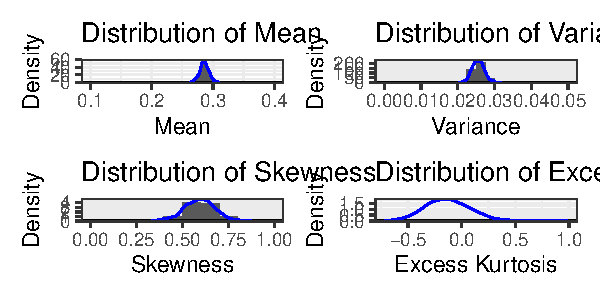
\includegraphics[width=\linewidth]{resampling.pdf}
\caption{Histograms for sampling distributions}
\label{fig:sampling}
\end{figure}

\section{Estimators (MOM and MLE)}


\section{Example (Death rates data)}


 You should objectively evaluate the evidence you found in the data. Do not embellish or wish-terpet (my made-up phase for making an interpretation you, or the researcher, wants to be true without the data \emph{actually} supporting it). Connect your findings to the existing information you provided in the Introduction.

Finally, provide some concluding remarks that tie together the entire paper. Think of the last part of the results as abstract-like. Tell the reader what they just consumed -- what's the takeaway message?

%%%%%%%%%%%%%%%%%%%%%%%%%%%%%%%%%%%%%%%%%%%%%%%%%%%%%%%%%%%%%%%%%%%%%%%%%%%%%%%%
% Bibliography
%%%%%%%%%%%%%%%%%%%%%%%%%%%%%%%%%%%%%%%%%%%%%%%%%%%%%%%%%%%%%%%%%%%%%%%%%%%%%%%%
\vspace{2em}

\noindent\textbf{Bibliography:} Note that when you add citations to your bib.bib file \emph{and}
you cite them in your document, the bibliography section will automatically populate here.

\begin{tiny}
\bibliography{bib}
\end{tiny}
\end{multicols}

%%%%%%%%%%%%%%%%%%%%%%%%%%%%%%%%%%%%%%%%%%%%%%%%%%%%%%%%%%%%%%%%%%%%%%%%%%%%%%%%
% Appendix
%%%%%%%%%%%%%%%%%%%%%%%%%%%%%%%%%%%%%%%%%%%%%%%%%%%%%%%%%%%%%%%%%%%%%%%%%%%%%%%%
\newpage
\onecolumn
\section{Appendix}

If you have anything extra, you can add it here in the appendix. This can include images or tables that don't work well in the two-page setup, code snippets you might want to share, etc.

\end{document}
